\chapter{Frequently Asked Questions - FAQ}

Here some general concepts and ideas are going to be explained, from good practices to programming advice or quick explanations.

\begin{itemize}
    %%%%%%%%%%%%%%%%%%%%%%%%%%%%%%%%%%%%%%%%%%%%%%%%%%%%%%%%%%%%%%%%%%%%%%%%%%%%%%%%%
    \item \textbf{How can I change the language of Visual Studio?}
    
    All this manual has been written taking into account that the IDE is configured in English, if you have used Spanish for the default language is possible to change it in \textit{Tools/Options/International Settings}. There are options and commands with no intuitive translation to Spanish so we recommend become familiarized with the English version of the IDE.
    
    %%%%%%%%%%%%%%%%%%%%%%%%%%%%%%%%%%%%%%%%%%%%%%%%%%%%%%%%%%%%%%%%%%%%%%%%%%%%%%%%%
    \item \textbf{What do I have to know about line Numbers?} 
    
    Why showing line numbers is useful can be clear, but there is a good practice that appears when our code is going to be shown in a text document (\LaTeX); it is useful to write before some subroutines, functions, etc. the line number in a comment inside the code in order to ``fix'' a position of the whole code and not move it when expanding the program. So when LaTeX looks for a code and extracts some lines, the result will always be the same. With the same purpose it is useful to leave some blank space between subroutine in order to expand them without moving the rest of the code.
    
    %%%%%%%%%%%%%%%%%%%%%%%%%%%%%%%%%%%%%%%%%%%%%%%%%%%%%%%%%%%%%%%%%%%%%%%%%%%%%%%%%
    \item \textbf{What are Static and Dynamic libraries? How can I create a \textit{.lib} file?} 
    
    Let's say we have some modules we feel comfortable about and we want to create a library with them, we have to choose kind. In a Static Library that code enters inside of the executable file once it is created, we could go to another computer and run that program without problem, we have also a quicker program as soon as it has all necessary code inside and doesn't have to look for outside. Disadvantages are; programs become heavier and if we find a bug in the library code, we will have to recompile all programs that use that lines. 
    
    Dynamic libraries are not in our executable file, so it is lighter and fixing bugs is easier as soon as it is repaired for all programs once we change just one file. However, we have to drag all libraries when moving the executable to another computer and the execution will be slower because of the search that program has to do when it needs those codes. We can see both have advantages and disadvantages and one or another will be used depending on the situation. Each of them is created, compiled and linked in a different way.
    
    We are going to see how to create a static library through an example:
    
    \begin{enumerate}
        \item We first create a project as seen before.
        \item Then we add the main file, and paste there this example code:
        
            \vspace{0.5cm}
            \lstinputlisting[language=Fortran, firstline=1, lastline=18]{Listing/Main.f90}
            
        \item Now we close our project (saving) and open a new one, but with kind \textit{Static Library} (\textit{File/New/Project.../Installed/Intel(R) Visual Fortran/Library/Static Library}). We take care of choosing name for the new solution (name of the library) and project and choosing location.
        \item We add to this Library project a \textit{.f90} file where we paste next example, this will be the module we save in our library:
            
            \newpage
            \vspace{0.5cm}
            \lstinputlisting[language=Fortran, firstline=12, lastline=27]{Listing/calculador_parametros_de_maquina.f90}
               
        \item Then we save all, compile the file and build the project. We can see that a .lib file (with the name of the project) and a \textit{.mod} file (with the name of the module) have appeared in the Release folder of the project.
        
            \vspace{0.5cm}
            \lstinputlisting[language=Fortran, firstline=29,    lastline=46]{Listing/calculador_parametros_de_maquina.f90}
        
        \item We can now close the solution of the library and open our project.
        \item Add to the project both files in the \textbf{Source folder}, using \textit{right click/Add/Existing Item/etc} for example. We can copy them first in our project folder and then include it from the IDE or link them to the original folder, this option let us rebuild the library whenever we want and our main project will be accessing always the latest version of the library but then Library Solution should not be opened in the IDE (I think).
        \item We build the project and run it without debugging. 
    \end{enumerate}
    
    There is an interesting result here, we obtain something like: 
        
    \begin{verbatim}
        Valor maximo  3.4028235E+38         
        Valor minimo  1.1754944E-38         
        Round_off     1.1920929E-07     
              
        Digitos significativos           6  
        Valor maximo  3.4028235E+38         
        Valor minimo  1.1754944E-38         
        Round_off     1.1920929E-07   
                
        Digitos significativos           6  
        1.1/2.        0.550000011920929       
        1.1/2         0.550000011920929     
        1.1/2d0       0.550000011920929     
        1.1d0/2d0     0.550000000000000     
        1.1e0/2e0     0.550000011920929     
        1/3d0         0.333333333333333     
        1./3d0        0.333333333333333     
        1d0/3d0       0.333333333333333     
        1d0/3.        0.333333333333333   
      \end{verbatim}

    This means that both ``real(4):: x'' and ``real :: y'' are being considered as simple precision, in order to make reals double precision by default we follow \ref{Configuration1} when building library and repeat the process. 
    
    %%%%%%%%%%%%%%%%%%%%%%%%%%%%%%%%%%%%%%%%%%%%%%%%%%%%%%%%%%%%%%%%%%%%%%%%%%%%%%%%%
    \item \textbf{What are Release and Debug?} 
    
    They are two possible configurations, each one with its settings, that allows to run the code in a different way. We can actually create more release modes (Debug modes, or the name we prefer) with a different solution and project configurations. We access the Configuration Manager by clicking on \textit{Build/Configuration Manager} or deploying the selector of Configuration (where it says Release and Debug), there we can create new options or edit those we have. For example, we could create one where default real KIND is 4 and other where is 8, by changing between Release modes we would run the code with the two behaviours (if we open the project options we directly can change between Modes and change options mode by mode).
    
    Debug mode will allow to run the code without optimiser turned on and lot of information will be included in the build files so we can check our program step by step, it can be useful for fixing bugs. However, if we are developing Numerical Simulations and related programs, we will use another kind of debugging; graphic assisted. Checking errors in the code starts with the printing of those results and the validation of the program module by module. That is why we include Dislin libraries in our program, to check quickly results and decide if we have executed correctly our program, later we will save the numerical results in order to plot them with another tool. 
    
    %%%%%%%%%%%%%%%%%%%%%%%%%%%%%%%%%%%%%%%%%%%%%%%%%%%%%%%%%%%%%%%%%%%%%%%%%%%%%%%%%
    \item \textbf{Do I have to \textit{Start without Debugging} my projects?} 
    
    We have seen what Debug and release are so we now understand why one of the IDE configuration (\ref{StartwD}) has been changing the command that starts the program, from the \textit{Start with Debugging} to this one, that goes directly to the execution of the code in the Release mode (or the mode selected).
    
    %%%%%%%%%%%%%%%%%%%%%%%%%%%%%%%%%%%%%%%%%%%%%%%%%%%%%%%%%%%%%%%%%%%%%%%%%%%%%%%%%
    \item \textbf{Which commands do I show in my IDE?} 
    
    Figure \ref{fig:Commands} shows some commands that are going to be highly used when programming. First two decrease and increase the indentation and next two comment and uncomment the code selected. Fifth one is the \textit{Start without Debugging} button already explained and the last buttons that are active compile and build our program. While the first compiles the current file, the second builds the project or library selected and last builds the whole solution (which we know can contain more than one project).
    
    \begin{figure}[h]
        \centering
        
\includegraphics[width= 0.9 \textwidth]{Figures/Commands}
        \caption{Very useful commands when programming, it is advisable to have them shown.}
        \label{fig:Commands}
    \end{figure}
    
    %%%%%%%%%%%%%%%%%%%%%%%%%%%%%%%%%%%%%%%%%%%%%%%%%%%%%%%%%%%%%%%%%%%%%%%%%%%%%%%%%
    \item \textbf{What should I know about navigation across files and codes?}
    
    There are some basic functionalities that are very useful when managing big codes; first one is the \textit{Navigate Backward} and \textit{Navigate Forward} buttons (Figure \ref{fig:Commands2}) which has the same function as Back and Forward in Windows OS but, instead of navigate across folders, we navigate across our opened and recently viewed codes. Even more powerful tools are \textit{Go To Definition} and \textit{Find All Differences} options. First we have to know how to activate them; we click on \textit{Tools/Options.../Text Editor/Fortran/Advanced} and we select \textit{True} in options \textit{Enable Find All References} and \textit{Enable Go To Definition} as seen in figure \ref{fig:Commands3}. 
    
    They are really useful tools; \textit{Go to Definition} allow us to find the declaration of any variable in our code, if we for example have a big program and we don't know what a variable is, we click with the right button of our mouse in the variable and click on that option, the window will automatically move to the line where is defined (or open a different module file and points the specific line). It can also open a new window with an specific file when we ask for the definition of a subroutine or a function and it's done in the same way. It doesn't work if the subroutine is in a module already compiled, library, etc. but if we have included the source in our project we will be able to navigate really quickly between those files.
    
    \textit{Find All References}, as the name says, will find in the whole project what we are asking for. If it's a variable we can know how many times (and where) it is used, changed, printed, etc. and if it is a subroutine we can find where it is called, and where it is defined for example. Once again we have to click on the right button in the name of the thing we want to look for and click in the option.
    
    \begin{figure}
        \centering
        
\includegraphics[width= 0.5 \textwidth]{Figures/Commands2}
        \caption{Navigation buttons.}
        \label{fig:Commands2}
    \end{figure}
    
    \begin{figure}
        \centering
        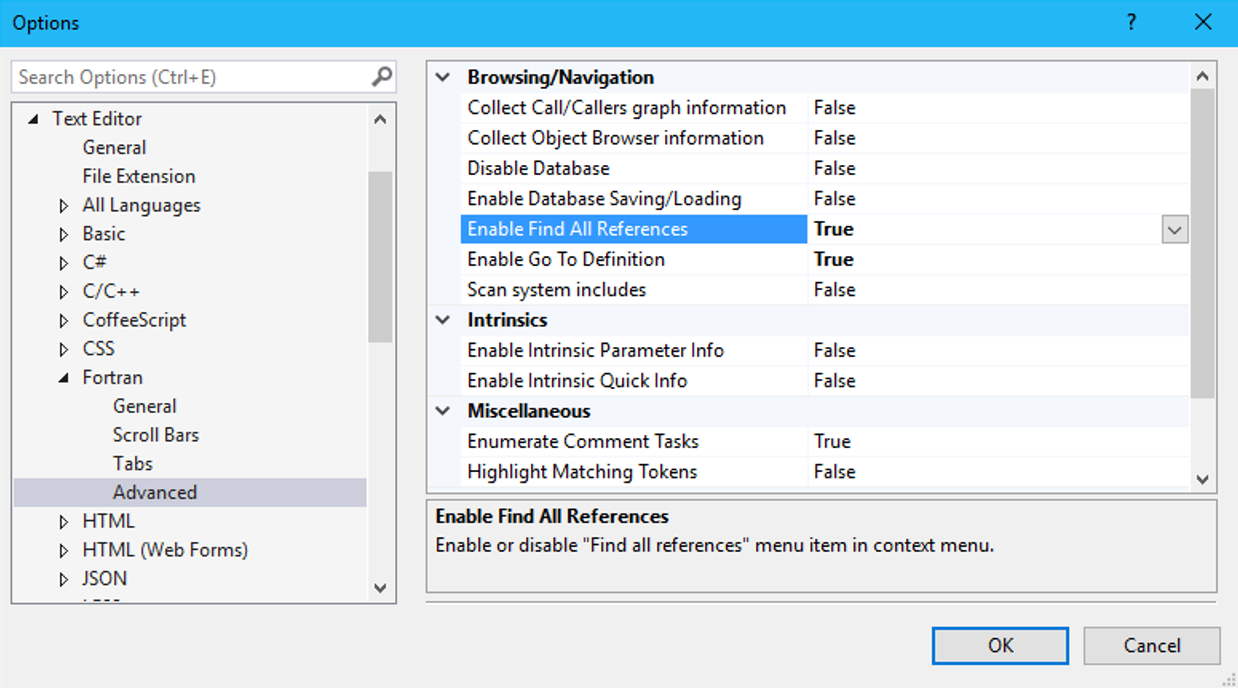
\includegraphics[width= \textwidth]{Figures/Commands3}
        \caption{Really interesting navigation options that will make the programming task easier.}
        \label{fig:Commands3}
    \end{figure}

    Related to this we can also remark that Visual Studio has a search engine that can be very useful to have shown in our toolbars, we've already seen how to do it before, the command is \textit{Find in files} or just \textit{Find} and also it can be minimized and put everywhere in the screen, ready to be used whenever.
    
    Finally, two extra options are \textit{Enable Intrinsic Parameter Info} and \textit{Enable Intrinsic Quick Info}, both can be found in \textit{Tools/Options.../Text Editor/Fortran/Advanced} also and should be activated (see figure \ref{fig:Commands4}). First ``displays the signature of an intrinsic in a tooltip when a user types the parameter list start character'', this means that information about the procedures and arguments will appear when typing a parenthesis after an intrinsic function or subroutine. Figure \ref{fig:Commands5} shows an example with the cosine function. Second option displays intrinsic information and descriptions when we place the pointer over an intrinsic name. Figure \ref{fig:Commands6} shows a list of arguments associated to the subroutine.
    
    \begin{figure}
        \centering
        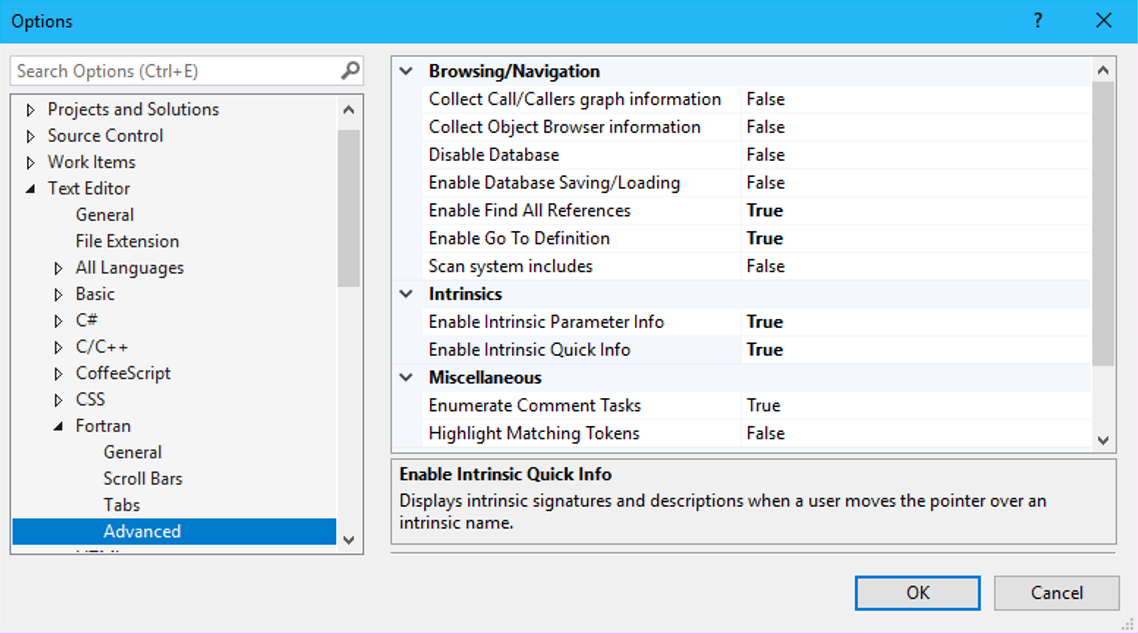
\includegraphics[width=  \textwidth]{Figures/Commands4}
        \caption{Extra options: \textit{Enable Intrinsic Parameter Info} and \textit{Enable Intrinsic Quick Info}, both really useful when our codes become long and they are spread in multiple source files.}
        \label{fig:Commands4}
    \end{figure}

    \begin{figure}
        \centering
        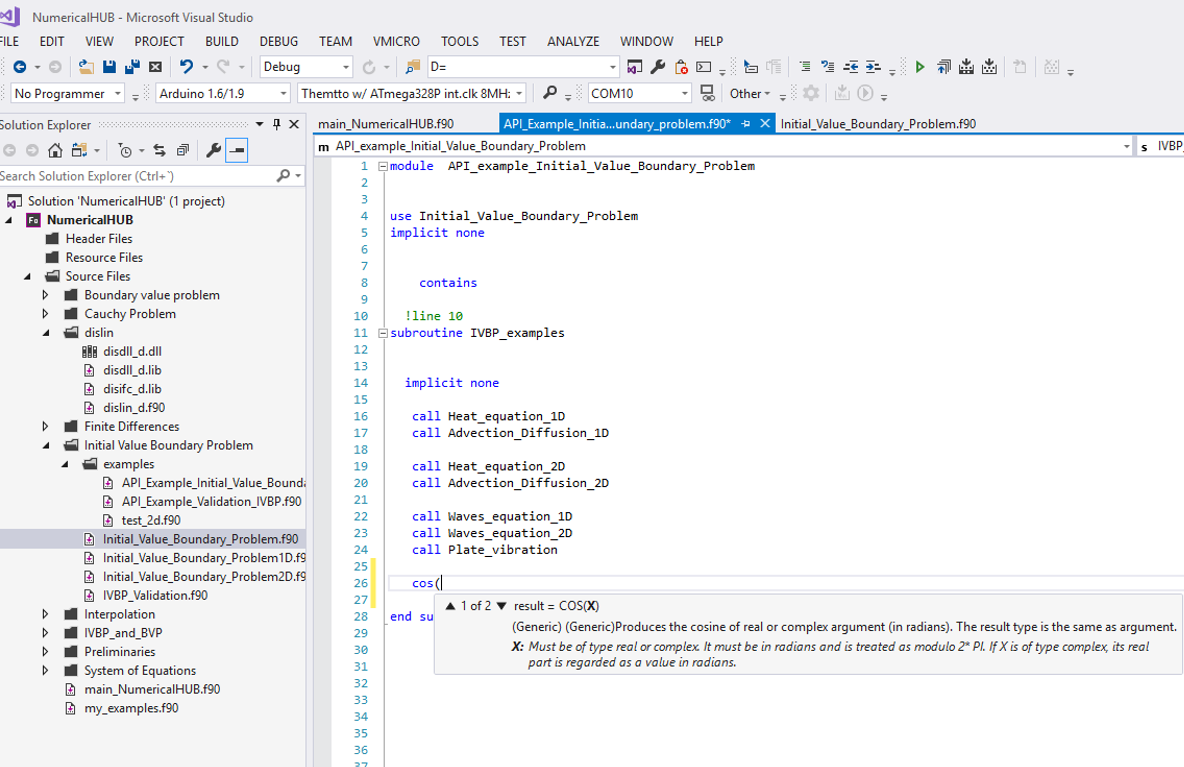
\includegraphics[width= \textwidth]{Figures/Commands5}
        \caption{Example of \textit{Intrinsic Parameter Info}.}
        \label{fig:Commands5}
    \end{figure}

    \begin{figure}
        \centering
        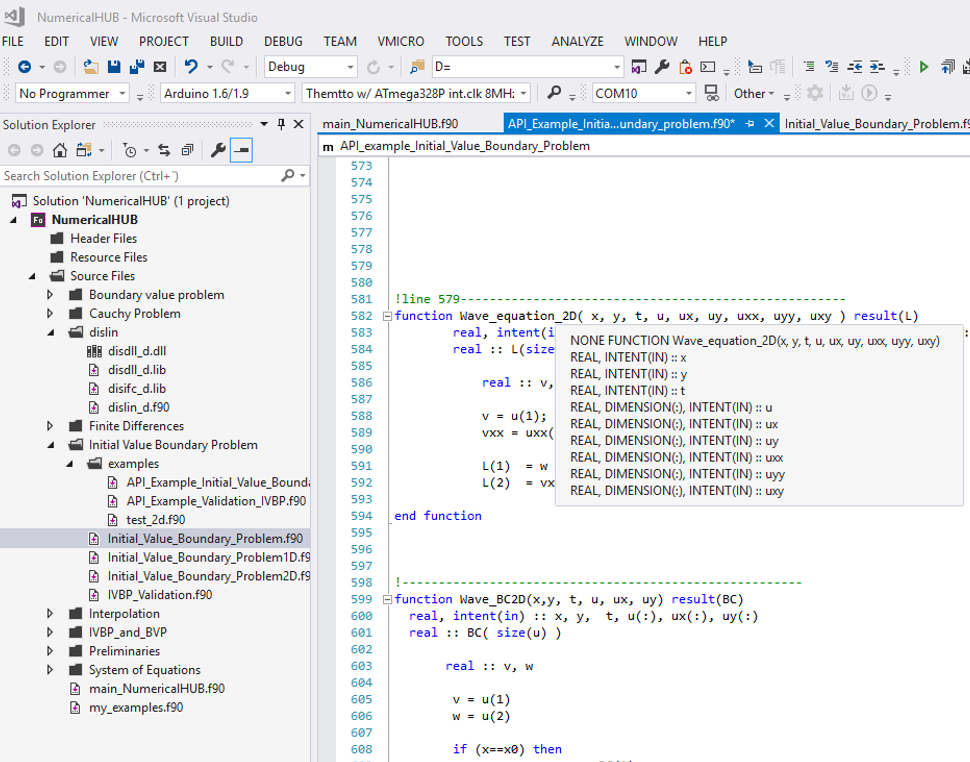
\includegraphics[width= \textwidth]{Figures/Commands6}
        \caption{Example of \textit{Intrinsic Quick Info}.}
        \label{fig:Commands6}
    \end{figure}
    
    \FloatBarrier
    %%%%%%%%%%%%%%%%%%%%%%%%%%%%%%%%%%%%%%%%%%%%%%%%%%%%%%%%%%%%%%%%%%%%%%%%%%%%%%%%%
    \item \textbf{What should I know about files and formats?}
    
    We have read in the introduction about source codes and object codes, the program we write needs of both codes, first one will be what we write with Fortran language and second will be the translation that the compiler makes in order to make them understandable for computers. The \textbf{source code} we write when using a programming language is stored in text files, in Fortran case those files has extension \textit{.f90}, \textit{.f} or \textit{.for} for example. 
    
    In order to execute that program we can choose between using an interpreter (it adapts the instructions while they are found in the code) or a compiler (translates the code to machine language), we are interested in compilers. It works developing two sub processes, first verifies that the source code is well written, fulfilling with syntactic and semantic Fortran rules, once finished, it creates an intermediate code called \textbf{object code} (with extension \textit{.obj} in Windows OS). Second sub process consists in linking the object code with other codes stored in libraries, the extensions used here are \textit{.dll} for shareable library files and \textit{.mod} for module files (created if a source file being compiled defines a Fortran module, which means, it uses MODULE statement). Finally the compiler optimize the code and converts it in an executable program (\textit{.exe} in Windows).
    
    The \textit{.mod} files has the interfaces of the modules that we have compiled, \textit{example.mod} contains the necessary information regarding the modules that have been defined in the program \textit{example.f90} and they are created with the \textit{.obj} file also, when compiling that project. Actually, a \textit{.mod} file is created for each module defined in our source (\textit{.f90}) file and a \textit{.obj} one will appear for the whole source. The module interfaces share the name with the modules and the object file has the same name as the source, typically, we can define one module in each file and assign the same name to the module and the source file (it's not a requirement but it helps to organize everything). More of this can be broaden in \citep{mod1}, \citet{mod2} and \citep{mod3}
    
    The history behind the file extensions of the source codes in Fortran can be broaden in \citet{f90} or \citet{f902}.
    
    Regarding Visual Studio files we can see \textit{.sln} which is the format where Visual stores our solution, there we open our projects associated. With the solution appears a configuration file with extension \textit{.suo}, as it is said in the on line manual of Visual Studio: 
    
    \begin{center}
        \begin{minipage}{0.7\linewidth}
            \vspace{5pt}        
            {\small
                ``The solution user options (\textit{.suo}) file contains per-user solution options. This file should not be checked in to source code control.
                
                The solution user options (\textit{.suo}) file is a structured storage, or compound, file stored in a binary format. You save user information into streams with the name of the stream being the key that will be used to identify the information in the \textit{.suo} file. The solution user options file is used to store user preference settings, and is created automatically when Visual Studio saves a solution.''
            }
            \begin{flushright}
                (\url {https://msdn.microsoft.com/es-es/library/bb165909.aspx})
            \end{flushright}
            \vspace{5pt} 
        \end{minipage}
    \end{center}
    
    Inside our solution folder we find folders with the different projects and the file with extension \textit{.vfproj} stores everything needed to open those projects. That specific extension makes reference to an Intel Fortran project file while, for example, \textit{.icproj} would be the file created for C++ compiler.
    
    More information about formats can be found in official documentation of Intel Fortran Compiler (\citep{format}), also in the manual \citep{manual} or in \citep{format2}. Figure \ref{fig:Formats} summarise some of the extensions used.
    
    \begin{figure}[h]
        \centering
        \caption{List with common file extensions used in Intel Fortran projects.}
        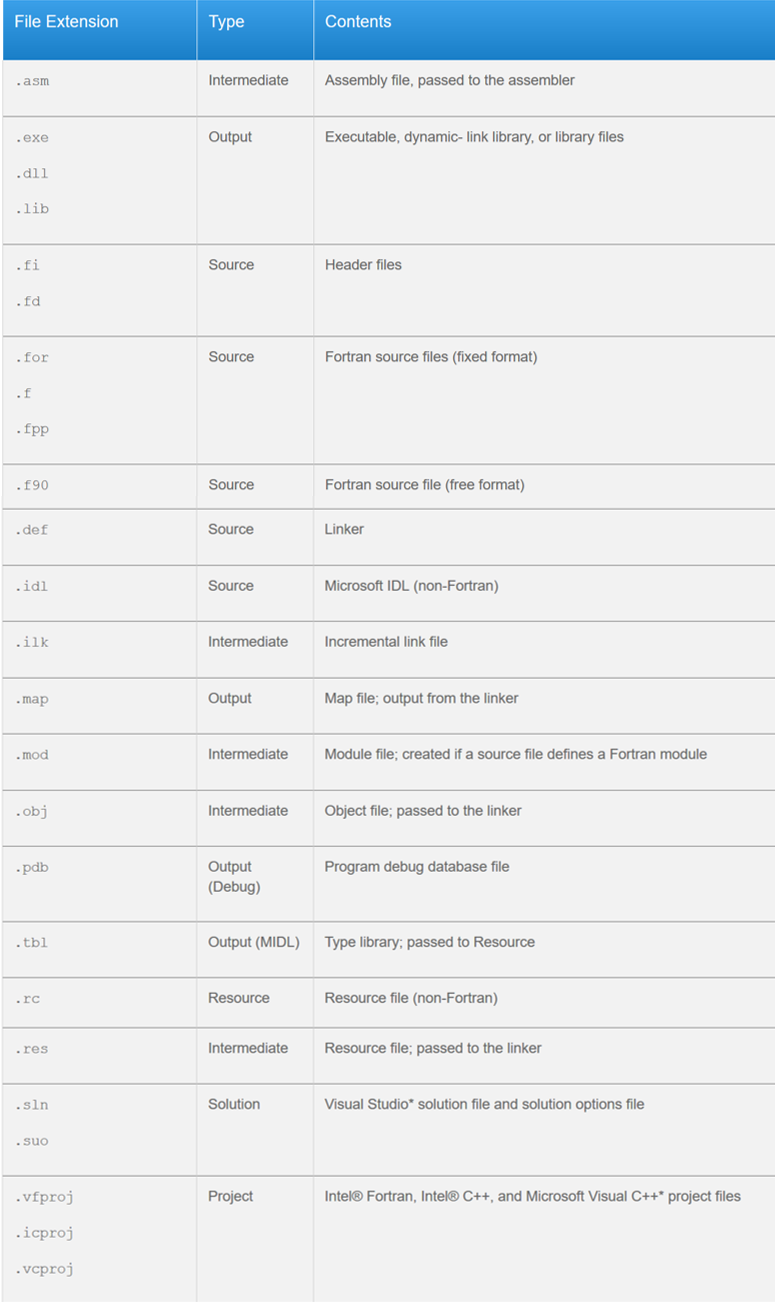
\includegraphics[width= 0.85 \textwidth]{Figures/Formats}
        \label{fig:Formats}
    \end{figure}
    
    %%%%%%%%%%%%%%%%%%%%%%%%%%%%%%%%%%%%%%%%%%%%%%%%%%%%%%%%%%%%%%%%%%%%%%%%%%%%%%%%%
     
    
\end{itemize}